\documentclass{article}
\usepackage[utf8]{inputenc}

\title{IF766 - Algoritmos De Aproximação}
\author{Pietro Bernardo Santos Masur}
\date{Novembro, 2019}

\usepackage{natbib}
\usepackage{graphicx}

\begin{document}

\maketitle

\section{Introdução}
Algoritmos de aproximação nos permitem obter soluções não exatas para problemas cuja resposta exata é impossível ou muito difícil de ser encontrada. Esse tipo de abordagem se enquadra dentro da grande área computacional de ciência da computação, na subárea de algoritmos. O uso de aproximações permite que uma grande quantidade de tempo e de poder computacional sejam economizados, sendo os resultados balizados para um erro percentual aceitável.
\begin{figure}[h!]
\centering
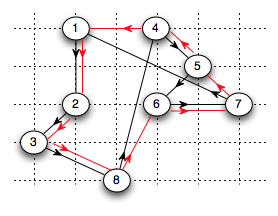
\includegraphics[scale=0.8]{pbsm.png}
\caption{Exemplo de algoritmo de aproximação, em vermelho.}\cite{Algoritmo}
\label{fig:Exemplo algoritmo}
\end{figure}

\section{Relevância}
\par
Para certos problemas de computação, de engenharia e de matemática (em especial os NP difíceis), são tão complexos que encontrar uma solução ótima se torna praticamente inviável. Entretanto, quase sempre é possível encontrar uma solução de optimização aproximada de maneira muito mais fácil. Nesse interim é que pode-se explicar a relevância dos algoritmos de computação.
\par
Um exemplo de aplicação do método aproximativo é o problema de como empacotar caixas num recipiente da maneira mais eficiente.\citep{VANSTEE2004535}
\section{Relação com outras disciplinas}
\par
As relações de algoritmos de otimização com outras disciplinas são virtualmente ilimitadas. Tanto em matemática quanto em engenharia, quanto nas mais diversas áreas da computação a otimização é sempre presente.\citep{wikipedia}

\bibliographystyle{plain}
\bibliography{pbsm}
\end{document}
